\chapter{Introduction}\label{intro}

\section{Overview}

Cancer is a genetic disease that for many years causes the highest number of global deaths \citep{Bray2021TheWorldwide}. Cancer development, or carcinogenesis, occurs as a consequence of a change in the normal cells that stimulate cell proliferation \citep{Weinberg1996HowArises}. This often forms tumours that damage the healthy part of the local tissues by invasion, increased infection, interference with the organ function and so on \citep{Tobias2014CancerManagement}. The process of carcinogenesis is complicated by the diversity in the forms cancer can possibly takes \citep{weinberg2013biology}. In particular, there are roughly 100 cancers that make up the major types: \gls{carcinoma}, \gls{lymphoma}, \gls{leukemia}, \gls{sarcoma} and \gls{neuroectodermal_tumour}. Cancer treatment relies on our understanding of the specific cancer sample. To illustrate, trastuzumab, which targets the \textit{HER2} protein, is known to provide good response in HER2-positive, but poor response in HER2-negative breast cancers \citep{Kreutzfeldt2020TheTherapies}. Another key to cancer treatment is early diagnosis and intervention \citep{Hawkes2019CancerDiagnosis}. For example, the 5-year survival rate for prostate cancer is 100\% \textit{v.s.} 48\% if diagnosed at stage 1 and 4, respectively. 

Genetically, the process of \gls{carcinogenesis} is operated and characterised by mutations \citep{Stratton2009}. In turn, whether a mutation occurs is determined by whether mutagens can form a \gls{lesion} in the DNA and whether the repair systems can correctly fix the lesion \citep{Chatterjee2017MechanismsMutagenesis}. While every cancer has a different set of mutations, certain mutation patterns have been found exclusive to several cancer types \citep{Alexandrov2013,Polak2015,Campbell2020}. Since all cancers originate from a normal cell \citep{Hanahan2011HallmarksGeneration}, the patterns of cancer \gls{mutagenesis} likely, to some extent, reflect the mutation tendency in the original cell type. During its development, the phenotype of a cancer sample could diverge from that of the original cell, but virtually all mutations prior to the divergence remain in the cancer genome (Figure \ref{fig:drivers_demo}). These divergence events can be caused by driver mutations, \textit{i.e.} mutations that promote cancer cell proliferation \citep{Pon2015}. An average cancer sample consists of only about 4-5 drivers, the rest are passenger mutations, which have neutral effects on the cancer progress \citep{Campbell2020}. Together, the whole history of mutations in a cancer sample helps characterise its mutation profile. 

\begin{figure}[h!]
    \centering
    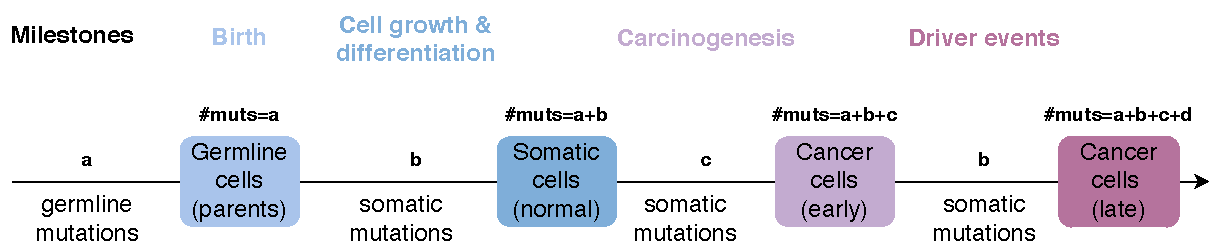
\includegraphics[scale=0.78]{graphics/drivers_demo.pdf}
    \caption{\textbf{Timeline of a carcinogenesis process.} Mutations are generally retained in the genome after each stage of carcinogenesis, even though carcinogenesis and driver events could change the phenotype of the cells. Together, all mutations available in a cancer cell make up it mutation profile. For the purpose of this project, only somatic mutations are considered because germline mutations occur prior to birth and are not the product of the environment of the differentiated cells in which cancer develop.}
    \label{fig:drivers_demo}
\end{figure}


The mutation profile reflects the mechanism of mutagenesis, which offers a great opportunity to study cancer. This project seeks to analyse the invaluable information extracted from the cancer mutation profile, with a hope that our enhanced understanding could potentially help guiding treatment. Furthermore, I seek to exploit this information to predict cancer types by training a \gls{classifier} that only relies on genomic sequencing data. In the long term, such a classifier could be an additional diagnostic tool to existing clinical approaches such as cytology or biopsy \citep{Stone1995Biopsy:Pitfalls}. In this era of next generation sequencing, liquid biopsies are gaining interest as a powerful non-invasive method for early cancer diagnosis because they involve screening for circulating tumour DNA in the blood rather than obtaining samples from a suspected local tissue \citep{Chen2019Next-generationDetection}. Developing a genome-based classifier model means that liquid biopsies could inform not only whether a cancer is present, but also where and what cancer is occurring at an early stage.  

Regarding the scope of the project, two aspects of of a cancer mutation profile were studied: where mutations tend to be found in the genome (hereafter the Genomic Location Effect, GLE) and what \gls{base} changes tend to be found in which genomic sequence context (hereafter the Sequence Context Effect, SCE). Secondly, the project is limited to point mutations, which are the most abundant type of mutations in cancer \citep{Alexandrov2020}. Thirdly, due to the different mutation rates between drivers and passengers, they should be considered separately - I focused on passenger mutations \citep{McFarland2014Tug-of-warProcesses}. Finally, I only investigated \glspl{sommut} as opposed to \glspl{germline_mut}, acknowledging that germline mutations could themselves be a risk factor of cancer. The reason for this is that germline mutations are present in effectively all the cells of a person, hence they are not the direct consequence of the mutagenic environment (Figure \ref{fig:drivers_demo}). 

To outline this chapter, section \ref{intro:gle} and \ref{intro:sce} review what is known about GLE and SCE, respectively. Section \ref{intro:ml} then briefly introduces the computational approaches used to study GLE and SCE, as well as how they can be used to train a machine learning classifier. Section \ref{intro:aims} then summarises the aims and hypotheses of the project. Section \ref{intro:findings} outlines the key findings.

\section{Genomic location effect (GLE)}
\label{intro:gle}
Certain regions of the genome are more prone to mutations than others, with the locations of these regions in the genome varying in different cell and cancer types \citep{Polak2015, Jiao2020}. This is believed to result from the fact that different cells have different chromatin structures \citep{Abascal2020ExpandedGenomes}, which determine how hidden DNA is in the chromatin complex across the genome. The accessibility of DNA to factors such as transcription, mutagens and repair systems can be measured by Dnase I hypersensitivity \citep[DHS;][]{Liu2019AApplications}. Highly accessible DNA means open chromatin status, and vice versa. Interestingly, it has been reported that open chromatin regions are less likely to harbour mutations than closed regions \citep{Polak2015,Prendergast2007ChromatinGenome}. Given that both \glspl{mutagen} and repairs determine whether mutations occur \citep{Ripley2001Mutation}, and that DNA is less accessible to both factors in closed regions, this suggests that the repair effect is generally stronger \citep[Figure \ref{fig:chromatin_demo};][]{Teng1997ExcisionSequences, Morse2002PhotoreactivationCerevisiae}. That said, the questions remain how strong chromatin structure is as a determinant of mutation genomic location, and whether there are other processes that influence how mutations are distributed across the genome. In addition, it is always equally intriguing to examine whether GLE, as a result of such determinants, can act as a distinct characteristic of the cancer mutation profile. 

\begin{figure}[h!]
    \centering
    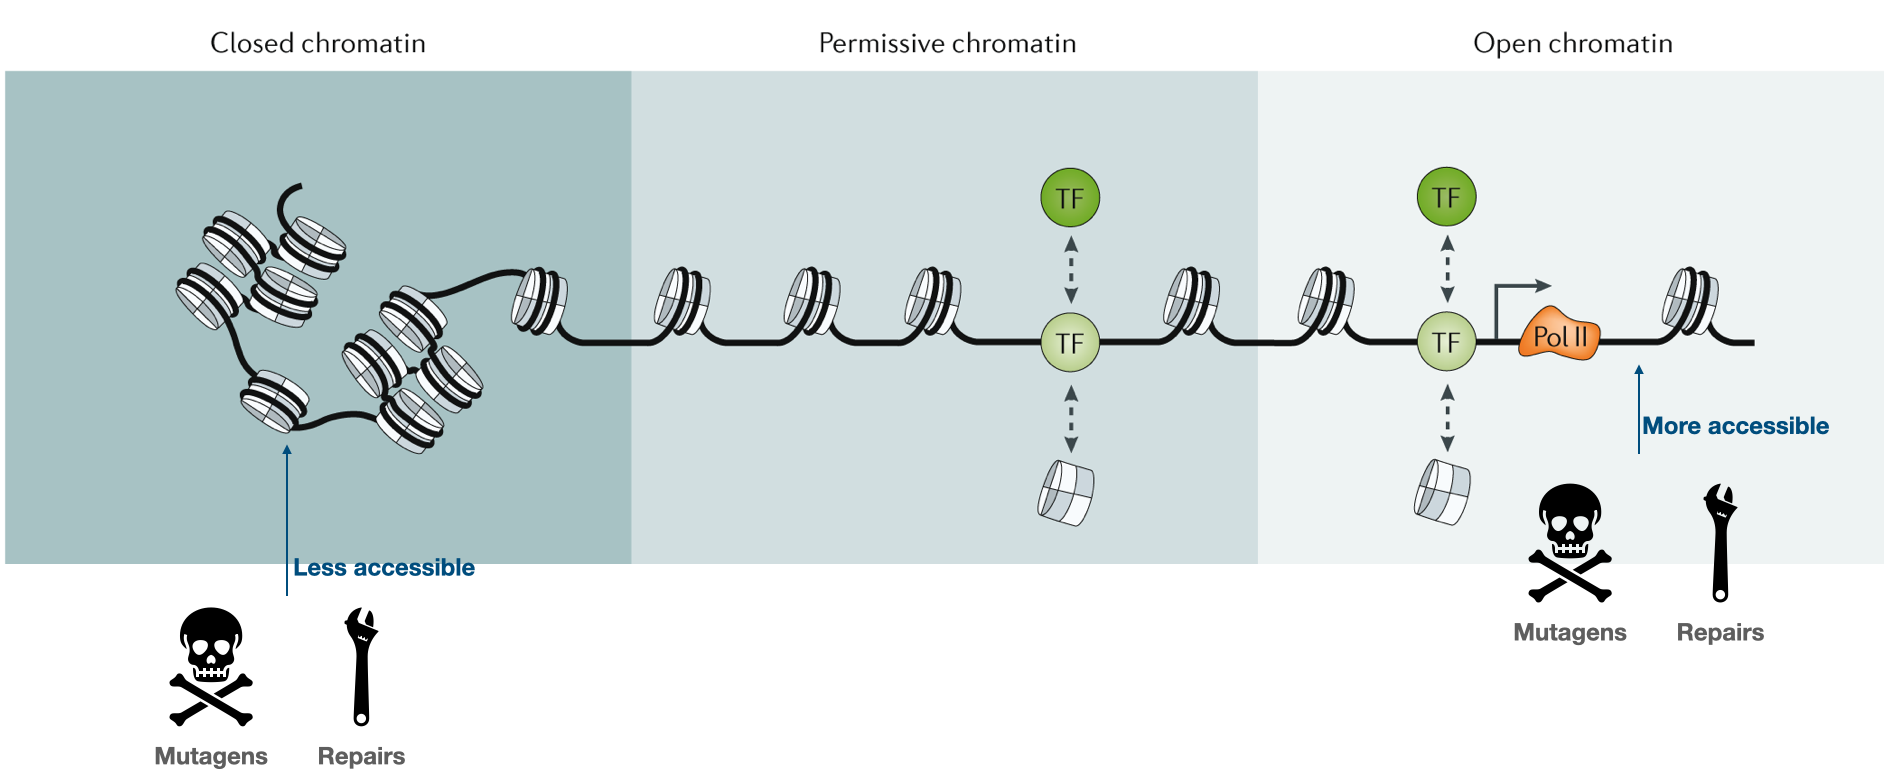
\includegraphics[scale=0.24]{graphics/chromatin_demo.png}
    \caption{\textbf{The distribution of mutations across the genome is hypothetically influenced by cell chromatin structure.} DNA in closed chromatin regions is not accessible to both mutagens and repairs, and is more prone to mutations. Different cell types have different chromatin structures as well as different repair systems, making genomic location effect (GLE) a potential factor that makes a cancer distinct from another. Figure modified from \citet{Klemm2019ChromatinEpigenome}. TF means transcription factor, Pol II means polymerase II}.
    \label{fig:chromatin_demo}
\end{figure}


To represent genomic location data, the convention is to count the number of mutations in a succession of 1 Mbp genomic segments, termed the bin method \citep{Kubler2019, Salvadores2019PassengerTumors, Chalmers2017AnalysisBurden, Salvadores2020MatchingPatterns}. However, the 1 Mbp size is picked by human, thereby imposing arbitrary boundaries to the genome. This leads to an unstable representation that is distorted when only slightly shifting the start of the bin boundaries (Figure \ref{fig:mutdistribution_demo}). As a result, my project experimented with smoothing GLE by estimating the \gls{density} at a genomic location based on the amount of data adjacent to it\footnote{details in }. The smooth representation assumes no rigid boundaries to the genome, thus less sensitive to the above pitfall. 
\begin{figure}[h!]
  \begin{minipage}[c]{0.45\textwidth}
    \caption{
      \textbf{In theory, the smoothing approach should be more robust than the bin approach.} Both panels depict the same mutation location data for a hypothetical chromosome, with the black dots below the x-axis representing the true location of mutations. By binning the genome by convention, one counts the number of mutations in each yellow bin. The obtained GLE data is then the yellow dots on top of each bin. This binned GLE data changes when shifting the bin boundaries from panel (a) to panel (b). Mutations on the right hand side of the last bin (10$^{th}$ bin) are forcefully removed. By smoothing the genome, GLE data is the same for both panels. The smoothing method also allows inclusion of mutations outside the last bins.
    } \label{fig:mutdistribution_demo}
  \end{minipage}\hfill
  \begin{minipage}[c]{0.52\textwidth}
    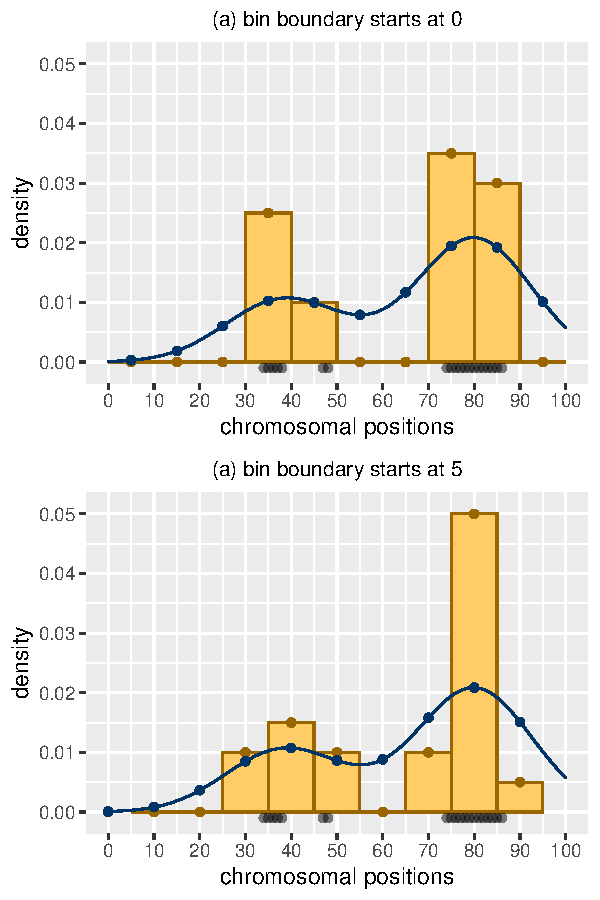
\includegraphics[width=\textwidth]{graphics/mutdistribution_demo.pdf}
  \end{minipage}
\end{figure}


\newpage
\section{Sequence context effect (SCE)}
\label{intro:sce}

Each cancer develops under the influence of different mutagenic processes, giving rise to diverse mutation compositions. These processes include, but are not limited to UV light \citep[known in skin melanoma;][]{Mohania2017}, the intrinsic cellular APOBEC deaminase activity \citep[\textit{e.g.} in B cells;][]{Kuppers2005MechanismsPathogenesis} and defective repairs \citep[\textit{e.g.} mutated \textit{BRCA} genes in breast cancer;][]{Navasardyan2021YY1TNBC}. \citet{Alexandrov2013, Alexandrov2020} showed that some processes were associated with certain mutation signatures. For instance, the signature SBS4, where there is an excess of C$\rightarrow$A mutations in the context of C[C$\rightarrow$A]A and C[C$\rightarrow$A]C over any other mutations, were only detected in tobacco smoke linked cancers such as liver hepatocellular carcinoma, lung adenocarcinoma and lung squamous cell carcinoma. As such, similar to \gls{gle}, SCE is also an important characteristic of the cancer mutation profile. 

In inspecting SCE, one should stay aware that mutations are usually closely linked with the \glspl{base} next to them \citep{Zhu2017}. A well known example is that the C$\rightarrow$T mutations tend to occur in the [C$\rightarrow$T]G context. One possible explanation is that proteins, be they repairs or mutagens, interact with DNA with high specificity (Figure \ref{fig:motif_demo}). There are two potential flaws to the standard way of representing SCE. First, while it is common practice to analyse mutation compositions in the 3-mer (3 base) context, evidence showed that bases beyond 3-mer could also influence the likelihood of mutations occurring \citep{Zhu2017,Zhu2020}. Second, base changes are generally assumed to be symmetric, meaning G$\rightarrow$A mutations are treated to be the same as their reverse complementary counterpart C$\rightarrow$T \citep{Alexandrov2013, Jiao2020}; but analyses in skin melanoma showed otherwise \citep{Zhu2017}. Accordingly, I seek to explore the information content available in different sequence context sizes, particularly outer positions to 3-mers; as well as the effect of strand symmetry/asymmetry in representing SCE.

\begin{figure}[h!]
    \centering
    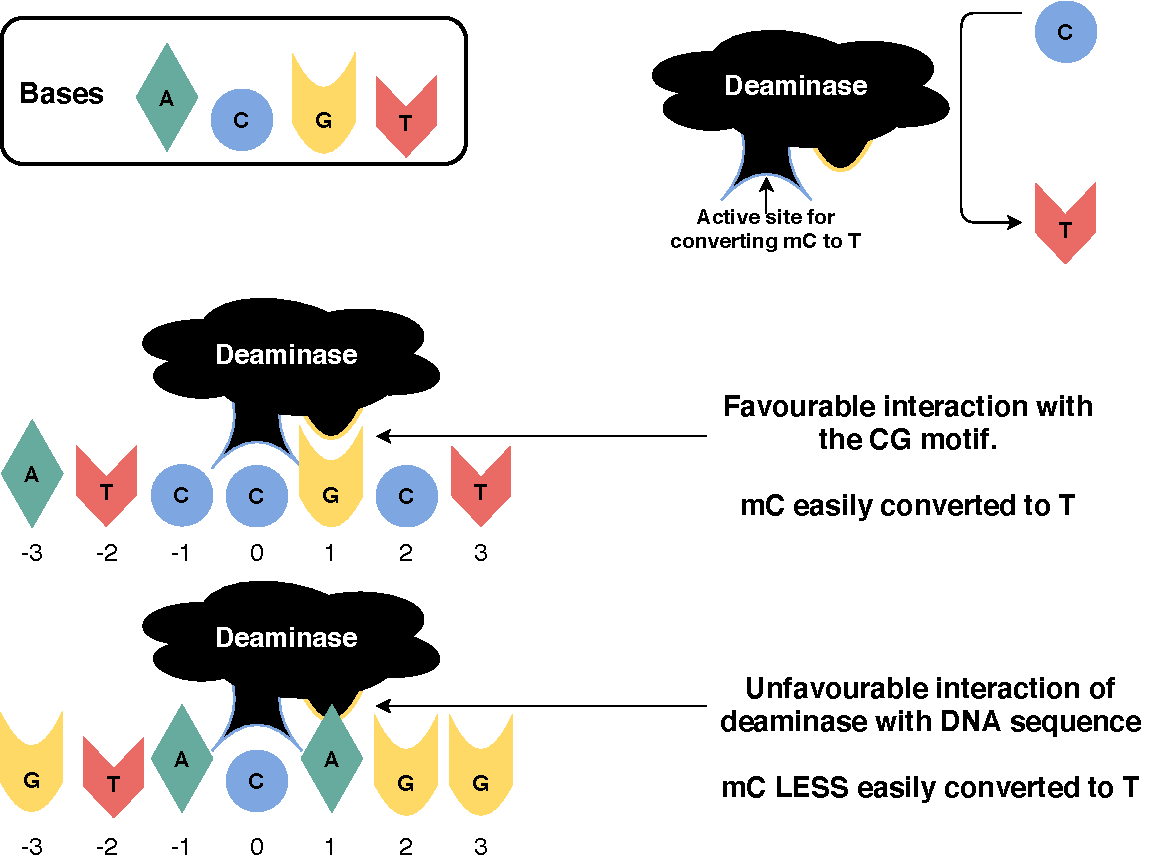
\includegraphics[scale=0.78]{graphics/motif_demo.pdf}
    \caption{\textbf{Mutations are closely linked with the bases next to them}. The schematic diagram depicts an example of hypothetical scenarios that could explain why this is the case. Here, a deaminase protein, which converts methylated C into T, interacts with DNA such that certain sequence contexts make the conversion more feasible than others. While many publications focus on the 3-mer context of mutations (pos -1, 0 and 1), which includes the base change and two bases immediately next to it, evidence shows that bases outside the 3-mer could still be influential. Part of this project seeks to explore the information content available in larger sequence contexts than 3-mers.}
    \label{fig:motif_demo}
\end{figure}


\section{Computational approaches to study GLE and SCE}
\label{intro:ml}

The release of the \gls{pcawg} project \citep{Campbell2020}, with whole genomic sequencing data for 2605 primary tumours of 38 cancer types, has made studying cancer genomics and developing cancer classification models on a large scale feasible. Nevertheless, analysing developing methods based on the PCAWG mutation data require satisfactory computational tools for data analysis. To do this, it is necessary to understand the nature of the data, which I approached on two levels, analysis on whole disease scale and classification on individual scale. First, data was investigated on the whole disease level (\gls{gle} in Chapter \ref{gle}; \gls{sce} in Chapter \ref{sce}). This means that for each cancer, mutations from all donors of that cancer were considered as a whole. This makes understanding the mutagenesis process easier as it magnifies the signals in the data if they are ``real''. Second, Chapter \ref{ml} trials different measures and data representations to train the classifiers on the individual donor level. The idea is that the more accurate the classifier, the better the assumptions imposed by its data representations could capture the nature of the data. The long term goal is to be able to apply the model to unseen data, such as the tumour genome of a new cancer patient. The analyses on two levels are complementary, in that they could be used to verify each other. Whereas whole disease analysis explores how and why a potential factor might be important, individual scale is a direct measure of how informative that factor is.  

\section{Aims and hypotheses}
\label{intro:aims}
\begin{itemize}
    \item To understand the tendency for mutations to be distributed across the genome. In particular, I seek to formally test whether mutations are distributed differently between closed and open chromatin regions; if so, how strong the bias towards closed chromatin regions is for each cancer. More importantly, I aim to investigate how informative GLE is as a result. As aforementioned, I expect if GLE is informative, then the smooth representation is the more efficient method to extract the information that the conventional bin representation.
    \item To understand how the information content available in the composition of mutations (SCE) is influenced by the base changes and their sequence contexts, especially the outer flanking positions of the 5-mer context. While it is very obvious to expect the base changes to be informative, I also expect some potential in the flanking positions. 
    \item To experiment with different measures and representations of GLE and SCE in order to improve the accuracy of the cancer classifier. This includes trialling smoothing \textit{v.s} binning GLE, different ways to integrate information from flanking bases to represent SCE, and the proposed asymmetric \textit{v.s.} the conventional symmetric representations of SCE. Finally, I examine whether combining SCE and GLE results in further accuracy improvement than each factor alone.  
\end{itemize}

\section{Key findings}
\label{intro:findings}
Overall, the project shows that both GLE and SCE are important characteristics of a cancer \gls{mut_profile}, manifesting in three aspects. First, mutations generally tend to occur in closed chromatin regions, but the degree of bias varies for different cancers. This suggests that chromatin structure is an important determinant of GLE, but there are other determining factors as well. Regardless of the driving forces, GLE was found to be distinctive of cancer types, particularly when the smoothing representation is used. Second, both components of SCE, the base changes and their sequence contexts are characteristic of cancers. Not surprisingly, information is more abundant closer to the mutations (3-mer), but the outer bases are also very informative. Additionally, there is more information in \glspl{transition} than in \glspl{transversion} for both base changes and their flanking bases. Third, when recruited to train classifiers, both GLE and SCE had a reasonably high predictive power by themselves, provided the data is represented appropriately. Specifically, as expected, smoothing GLE in any form provided a higher predictive power than binning it. Regarding SCE, incorporating the immediate neighbours within the 3-mer neighbourhood improved accuracy over the base changes alone. Moreover, classifier performance was improved when omitting the traditional assumption of strand symmetric mutations. Interestingly, while information was detected in the outer bases of the 5-mer sequence context, incorporating this information into the classifier appeared to be quite challenging. Finally, even though GLE and SCE were expected to be separate sources of information, SCE seemed to be the predominating contributor of the classifier. When training the model, I identified the problem of imbalanced design, which needs to be addressed in future research.   

